
% Can also go beyond and define dynamical quantum $SU(n,1)$, starting from one-parameter space of complex projective spaces. Works for all hermitian symmetric spaces


%The relations for the adjoint further imply that \begin{eqnarray*}u_{kl}^{+-} &=&\frac{E(l,l-1)}{E(k,k+1)}(u_{k+1,l-1}^{-+})^*,\\  u_{kl}^{++}&=& \frac{E(l,l+1)}{E(k,k+1)}(u_{k+1,l+1}^{--})^* .\end{eqnarray*}


%\begin{eqnarray*} u_{++} &=& \frac{w_+(\rho)^{1/2}}{w_+(\lambda)^{1/2}}u_{--}^*,\\u_{+-}&=& (-1)^{s_q}  \frac{w_-^{1/2}(\rho)}{w_+^{1/2}(\lambda)}u_{-+}^*.  \\ 
%\end{eqnarray*}

%Let us write \[F(k) = |q|^{-1}w_+(k) =  |q|^{-1}\frac{|q|^{x+k+1}+|q|^{-x-k-1}}{|q|^{x+k}+|q|^{-x-k}},\] and further put\[\alpha = \frac{F^{1/2}(\rho-1)}{F^{1/2}(\lambda-1)}u_{--},\qquad \beta = \frac{1}{F^{1/2}(\lambda-1)}u_{-+}.\] Then the unitarity of $(u_{\epsilon,\nu})_{\epsilon,\nu}$ together with \eqref{EqAdju} and \eqref{EqGradu} are equivalent to the commutation relations \begin{equation}\label{EqqCom} \alpha \beta = qF(\rho-1)\beta\alpha \qquad \alpha\beta^* = qF(\lambda)\beta^*\alpha\end{equation} \begin{equation}\label{EqDet} \alpha\alpha^* +F(\lambda)\beta^*\beta = 1,\qquad \alpha^*\alpha+q^{-2}F(\rho-1)^{-1}\beta^*\beta = 1,\end{equation}\begin{equation*} F(\rho-1)^{-1}\alpha\alpha^* +\beta\beta^* = F(\lambda-1)^{-1},\qquad  F(\lambda)\alpha^*\alpha +q^{-2}\beta\beta^* = F(\rho),\end{equation*} \begin{equation}\label{EqGrad} f(\lambda)g(\rho)\alpha =
%\alpha f(\lambda+1)g(\rho+1),\qquad f(\lambda)g(\rho)\beta = \beta f(\lambda+1)g(\rho-1).\end{equation}%layout might be nicer

%These are precisely the commutation relations for the dynamical quantum $SU(2)$-group as in \cite[Definition 2.6]{KoR1}, except that the precise value of $F$ has been changed by a shift in the parameter domain by a complex constant. Clearly, by Theorem \ref{TheoGenRel} the (total) coproduct on $A_x$ also agrees with the one on the dynamical quantum $SU(2)$-group, namely \begin{eqnarray*} \Delta(\alpha) &=& \Delta(1) (\alpha\otimes \alpha - q^{-1}\beta\otimes \beta^*),\\ \Delta(\beta) &=& \Delta(1)(\beta\otimes \alpha^* +\alpha\otimes \beta)\end{eqnarray*} where $\Delta(1) = \sum_{k\in \Z} \rho_k\otimes \lambda_k$.

%Let us write $B_x = B_x(\Gamma)$ for the $*$-algebra generated by a copy of the $*$-algebra $c_b(\Z\times \Z)$ of bounded functions on $\Z\times \Z$ as well as elements $\alpha,\beta$ satisfying the relations \eqref{EqqCom}, \eqref{EqDet} and \eqref{EqGrad}.

% Lemma doesn't work because $\alpha$,$\beta$ not bounded.
%\begin{Lem} There is a one-to-one correspondence between non-degenerate $*$-representations of $A_x$ on Hilbert spaces and unital $^*$-representations of $B_x$ on Hilbert spaces for which the restriction to $c_b(\Z\times \Z)$ is strictly continuous.
%\end{Lem}


% Give motivation for result coamenability: continuous spectrum can only be in [-2,2], and easy to see universal one has bigger cont. spectrum
\section{The C$^*$-algebras of the dynamical quantum $SU(2)$}\label{SecUni}

\subsection{Definition}\label{SecDefSUqdyn}

We assume in the following that $0<q<1$, and we choose also $x>0$.
%We also choose $x\in \lbrack \sqrt{q},1\rbrack$.

We recall from \cite[Section 5]{DCT1} the definition of the dynamical $SU(2)$ partial compact quantum group $SU_{q,x}^{\dyn}(2)$, whose associated partial Hopf $^*$-algebra we denote by $(A_x,\Delta)$. Denote $\ctau(y) = y+y^{-1}$ and $w_{\pm}(y) = \frac{\ctau(q^{\pm 1}y)}{\ctau(y)}$. Let $\Lambda_x = xq^{\Z}$, and let $B$ be the $^*$-algebra of finite support functions on $\Lambda_x\times \Lambda_x$, whose Dirac functions we write as $\delta_{(y,z)}=\UnitC{y}{z}$. Then $A_x$ is the $^*$-algebra generated by a copy of $B$ and elements \[(u_{\epsilon,\nu})_{y,z}\] for $\epsilon,\nu\in \{-1,1\}=\{-,+\}$ and $y,z\in \Lambda_x$ with defining relations \begin{eqnarray*} \sum_{\mu\in \{\pm\}} (u_{\mu,\epsilon})_{q^{-\mu}w,y}^* (u_{\mu,\nu})_{q^{-\mu}w,z}&=& \delta_{\epsilon,\nu} \delta_{y,z} \UnitC{w}{q^{\epsilon}y},\\ \sum_{\mu\in \{\pm\}} (u_{\epsilon,\mu})_{y,w} (u_{\nu,\mu})_{z,w}^* &=& \delta_{\epsilon,\nu}\delta_{y,z} \UnitC{y}{w} \\ (u_{\epsilon,\nu})_{y,z}^* &=& \frac{\nu w_{\nu}(z)^{1/2}}{\epsilon w_{\epsilon}(y)^{1/2}} (u_{-\epsilon,-\nu})_{q^{\epsilon}y,q^{\nu}z}.\end{eqnarray*} The element $(u_{\epsilon,\nu})_{y,z}$ lives inside the component $\Gr{(A_x)}{y}{q^{\epsilon}y}{z}{q^{\nu}z}$.

Consider $M(A_x)$, the multiplier algebra of $A_x$. For a function $f$ on $\Lambda_x\times \Lambda_x$, write $f(\lambda,\rho) = \sum_{y,z} f(y,z)\UnitC{y}{z} \in M(A_x)$. Similarly, for a function $f$ on $\Lambda_x$ we write $f(\lambda) = \sum_{y,z} f(y)\UnitC{y}{z}$ and $f(\rho) = \sum_{y,z}f(z)\UnitC{y}{z}$. We then write for example $f(q\lambda,\rho)$ for the element corresponding to the function $(y,z)\mapsto f(qy,z)$.

We can further form in $M(A_x)$ the elements $u_{\epsilon,\nu} = \sum_{y,z} (u_{\epsilon,\nu})_{y,z}$. Then $u=(u_{\epsilon,\nu})$ is a unitary 2$\times$2 matrix. Moreover, \begin{equation}\label{EqAdju}u_{\epsilon,\nu}^* = u_{-\epsilon,-\nu}\frac{ \nu w_{\nu}^{1/2}(\rho)}{\epsilon w_{\epsilon}^{1/2}(\lambda)}.\end{equation} We have the following commutation relations between functions on $\Lambda_x\times \Lambda_x$ and the entries of $u$: \begin{equation}\label{EqGradu} f(\lambda,\rho)u_{\epsilon,\nu} = u_{\epsilon,\nu}f(q^{-\epsilon}\lambda,q^{-\nu}\rho).\end{equation}

In the following, we will write $u_{--}=\alpha, u_{-+}= \beta, u_{+-}=\gamma,u_{++}=\delta$. These satisfy the following relations.

\begin{equation}\label{EqId1}\left\{\begin{array}{lllllll} \alpha\alpha^* + \beta\beta^*, &=& 1 &&  \gamma\gamma^* + \delta\delta^* &=& 1,\\ \alpha^*\alpha+ \gamma^*\gamma &=&1,&&\beta^*\beta+ \delta^*\delta &=& 1,\\ \\ \alpha \gamma^* = -\beta \delta^*, &&&& \alpha^*\beta = -\gamma^*\delta, \end{array}\right.\end{equation}

\begin{equation}\label{EqId2} \delta^* = \alpha \frac{w_+^{1/2}(\rho)}{w_+^{1/2}(\lambda)}, \quad \gamma^*=  - \beta\frac{w_{-}^{1/2}(\rho)}{w_+^{1/2}(\lambda)},\quad  \beta^* = - \frac{w_+^{1/2}(\lambda)}{w_{-}^{1/2}(\rho)}\gamma, \quad  \alpha^* =  \frac{w_+^{1/2}(\lambda)}{w_+^{1/2}(\rho)}\delta.\end{equation}

The total coproduct $\Delta$ on $A_x$ is completely determined by the formula \[\Delta(u_{\epsilon,\nu}) = \Delta(1)\left(\sum_{\mu} u_{\epsilon,\mu}\otimes u_{\mu,\nu}\right).\]

%As before, the counit $\epsilon$ gives a $^*$-representation $\weps:A_x \rightarrow B(l^2(\Lambda_x))$ which can again be uniquely characterised, using its extension to $M(A_x)$, by 

%\begin{align*} \weps(\alpha) \delta_y = \delta_{qy},&& \weps(\beta) = 0,&&\weps(f(\lambda,\rho))\delta_y = f(y,y)\delta_y.\end{align*}

%Finally, the antipode $S$ is determined by $S(u_{\epsilon,\nu}) = u_{\nu,\epsilon}^*$ and $S(f(\lambda,\rho)) = f(\rho,\lambda)$. 

% Next piece only for $\sigma = +$!


For completeness, let us also recall the correspondence with the formalism of Koelink and Rosengren \cite{KoR1}. Let us index the generators as they appear in \cite[Definition 2.6]{KoR1} by KR. Moreover, we shift in all their formulas the parameters $\mu$ and $\lambda$ by $\frac{i\pi}{2\ln(q)}$, and after this shift use on $\mathfrak{h}^* \cong \C$ the ordinary complex conjugation as the abstract conjugation $\lambda \mapsto \bar{\lambda}$, cf.~ the discussion before \cite[Definition 2.8]{KoR1}. Then with $F(y) = \frac{q^{2(y+1)}+q^{-2}}{q^{2(y+1)}+1}$ denoting the (shifted) function appearing at the beginning of section 2.2 in \cite{KoR1}, we have that the correspondence \begin{align*} &\lambda = q^{\lambda_{KR}+1},&& \rho = q^{\mu_{KR}+1},\\ &\alpha = \frac{F^{1/2}(\lambda_{KR}-1)}{F^{1/2}(\mu_{KR}-1)}\alpha_{KR}&& \beta = F^{1/2}(\lambda_{KR}-1)\beta_{KR},\\ &\gamma = F^{-1/2}(\mu_{KR}-1)\gamma_{KR}&& \delta = \delta_{KR}\end{align*} respects the commutation relations of all the generators. 

The identities in the next lemma follow immediately from \eqref{EqId1} and \eqref{EqId2}.

\begin{Lem} The following identities hold in $M(A_x)$. \begin{eqnarray}\label{EqId3} \tau(\lambda)\tau(q\rho)\alpha^*\alpha -\tau(\lambda/q)\tau(\rho)\alpha\alpha^* &=& (q-q^{-1})(\lambda\rho-1/\lambda\rho) \\
 \label{EqId4} \tau(\lambda)\tau(\rho/q) \beta^*\beta - \tau(\lambda/q)\tau(\rho) \beta\beta^* &=& (q-q^{-1})(\lambda/\rho-\rho/\lambda) \\  
  \tau(\lambda)\tau(q\rho)\gamma^*\gamma -\tau(q\lambda)\tau(\rho)  \gamma\gamma^* &=& (q-q^{-1})(\lambda/\rho-\rho/\lambda) \\
 \tau(\lambda)\tau(\rho/q)\delta^*\delta - \tau(q\lambda)\tau(\rho)\delta\delta^*   &=&  (q^{-1}-q)(\lambda\rho-1/\lambda\rho) 
 \end{eqnarray}


\end{Lem} 

\subsection{Representation theory of $A_x$}

We wish to classify the irreducible $^*$-representations of $A_x= \Pol(SU_{q,x}^{\dyn}(2))$. Our method will be based on a \emph{decoupling} of $A_x$. For this, we need to recall the definition of the \emph{quantized enveloping algebra of $\su(1,1)$}. % Add ref.

\begin{Def} Let $q>0$. The \emph{quantized enveloping algebra $U_q(\su(1,1))$} is the universal unital $^*$-algebra generated by elements $E,F,K,K^{-1}$ satisfying the following commutation rules: 
\begin{itemize}
\item $K^{-1}$ is the inverse of $K$, 
\item $K^* = K$ and $E^* = F$, 
\item $KE = qEK$,
\item $\lbrack F,E\rbrack = \frac{K^2-K^{-2}}{q-q^{-1}}$.
\end{itemize}
\end{Def}

One can turn $U_q(\su(1,1))$ into a Hopf $^*$-algebra, but this extra structure will not be needed. 

It will be convenient to consider a slight variation of $U_q(\su(1,1))$ by formally adding support projections of $K$, cf. \cite[Chapter 23]{Lus1}. We will write $\Gamma_y = yq^{\frac{1}{2}\Z}$  for $y>0$.

%E_r = E1_r, F_r = 1_rF$
\begin{Def} Let $y>0$. We define $U_q^{\Gamma_y}(\su(1,1))$ to be the (non-unital) $^*$-algebra generated by a copy of the $^*$-algebra of finite support functions on $\Gamma_y$, whose Dirac functions we will write $\Unit_r$, together with elements $E_{r},F_r$ for each $r\in \Gamma_y$, such that $E_{r}^* = F_{r}$ and 
\begin{itemize}
\item $\Unit_{qr}E_{r} = E_{r} = E_{r}\Unit_{r}$, 
\item $\Unit_r F_r = F_r  = F_r\Unit_{qr}$
\item $F_{r}E_{r} - E_{r/q}F_{r/q}  = \frac{r^2-r^{-2}}{q-q^{-1}} \Unit_{r}$.
\end{itemize}
\end{Def} 

\begin{Lem} We have a unique $^*$-homomorphism $U_q(\su(1,1))\rightarrow M(U_q^{\Gamma_y}(\su(1,1)))$ such that \[K \mapsto \sum_{r\in \Gamma_y} r\Unit_r,\quad E\mapsto \sum_{r\in \Gamma_y} E_{r},\quad F\mapsto \sum_{r\in \Gamma_y} F_r. \] Moreover, this $^*$-homomorphism is injective.
\end{Lem} 
\begin{proof} It is clear that the images are well-defined multipliers. It is then immediate that there is a unique $^*$-homomorphism with the above prescribed images.

Let us show that it is injective. Consider the vector space $V$ with basis $\{e_n\mid n\in \N\}$. Then we can represent $U_q^{\Gamma_y}(\su(1,1))$ on $V$ (neglecting the $^*$-structure) by \[\Unit_r e_n = \delta_{r,yq^n}e_n,\quad E_{r} e_n = \delta_{r,yq^n} e_{n+1},\]\[(q-q^{-1})^2 F_{r}e_n = \delta_{r,yq^{n-1}} (q^n-q^{-n})(q^{n-1}y^2-q^{1-n}y^{-2})e_{n-1}.\] This representation can then be extended to the multiplier algebra. As the elements $E^mK^nF^l$ form a basis of $U_q(\su(1,1))$, it follows that the above representation is injective when considered as a $U_q(\su(1,1))$-represention via the $^*$-homomorphism in the lemma, which implies its injectivity.
\end{proof}  

In what follows, we will need two copies of $U_q(\su(1,1))$. We will correspondingly use the indices $(1)$  and $(2)$ as upper indices for the generators of the two copies.
\begin{Lem} 

There is a unique non-degenerate $^*$-homomorphism \[\Phi: U_q^{\Gamma_x}(\su(1,1))\otimes U_q^{\Gamma_1}(\su(1,1))\rightarrow A_x\] such that 
\[(q^{-1}-q)\Phi(E^{(1)})=  \alpha \tau^{1/2}(\lambda)\tau^{1/2}(q\rho),\qquad (q^{-1}-q)\Phi( E^{(2)}) =  \beta \tau^{1/2}(\lambda)\tau^{1/2}(\rho/q),\]
\[(q^{-1}-q)\Phi(F^{(1)})=  \delta\tau^{1/2}(\lambda)\tau^{1/2}(\rho/q),\qquad (q^{-1}-q)\Phi( F^{(2)}) =  - \gamma\tau^{1/2}(\lambda)\tau^{1/2}(q\rho),\]
\[\Phi(\Unit_r^{(1)}) = \sum_{z\in \Lambda_x} \UnitC{r^2/z}{z},\qquad \Phi(\Unit_s^{(2)}) = \sum_{z\in \Lambda_x} \UnitC{s^2z}{z}.\] Moreover, $\Phi$ is surjective.
\end{Lem} 

\begin{proof} Note first that the values for $\Phi(E^{(i)})$ and $\Phi(F^{(i)})$ given above are well-defined inside $M(A_x)$, with $\Phi(F^{(i)})^* = \Phi(E^{(i)})$. We can then define $\Phi(E^{(i)}_r) = \Phi(E^{(i)})\Phi(\Unit_r^{(i)})$ and $\Phi(F^{(i)}_r) = \Phi(\Unit_r^{(i)})\Phi(F^{(i)})$. 

It is  easily verified that $\Phi(\Unit_{qr}^{(i)})\Phi(E^{(i)}_r) = \Phi(E^{(i)}_r) = \Phi(E^{(i)}_r)\Phi(\Unit_r^{(i)})$ and $\Phi(\Unit_r^{(i)})\Phi(E^{(i+1)}_s) = \Phi(E^{(i+1)}_s)\Phi(\Unit_r^{(i)})$ (with the upper indices taken modulo 2).

Let us now verify that $\lbrack \Phi(E^{(i)}_r)^*,\Phi(E^{(i)}_r)\rbrack = \frac{r^2-r^{-2}}{q-q^{-1}}\Phi(\Unit_r)$. This follows immediately from \eqref{EqId3} and \eqref{EqId4}.

It remains to check that $\lbrack \Phi(E^{(1)}_r),\Phi(E^{(2)}_s)\rbrack = 0$ and $\lbrack \Phi(E^{(1)}_r)^*,\Phi(E^{(2)}_s)\rbrack = 0$, but these identities are equivalent with the last two identities in \eqref{EqId1}.

Finally, $\Phi(\Unit_r^{(1)}\Unit_s^{(2)}) = \UnitC{rs}{r/s}$ whenever $r/s\in \Lambda_x$, and it follows that the image of $\Phi$ contains all finite support functions on $\Lambda_x\times \Lambda_x$. It is then clear that in fact $\Phi$ is surjective. 
\end{proof}

Let $C = (q^{-1}-q)^2FE-qK^2-q^{-1}K^{-2}$ be the Casimir element of $U_q(\su(1,1))$. It  is a self-adjoint element generating its center. 

\begin{Lem}\label{LemKer} The kernel of $\Phi$ is generated by all $(C^{(1)}+C^{(2)})\Unit_r^{(1)}\Unit_s^{(2)}$, and all $\Unit_r^{(1)}\Unit_s^{(2)}$ with $rs\notin \Lambda_x$
\end{Lem} 
\begin{proof} Let $\widetilde{B}_x$ be the quotient of $B_x = U_q^{\Gamma_x}(\su(1,1))\otimes U_q^{\Gamma_1}(\su(1,1))$ by the ideal generated by $(C^{(1)}+C^{(2)})B_x$ and all $\Unit_r^{(1)}\Unit_s^{(2)}$ with $rs\notin \Lambda_x$. It is straightforward to compute that $\Phi$ descends to a homomorphism $\widetilde{\Phi}$ on $\widetilde{B}_x$. 

Denote the images of the generators of $B_x$ in $\widetilde{B}_x$ by the same symbols adorned with a tilde. For $w,z\in \Lambda_x$, write $\widetilde{\Psi}(\UnitC{w}{z}) = \widetilde{\Unit}_{\sqrt{wz}}^{(1)}\widetilde{\Unit}_{\sqrt{w/z}}^{(2)}$, and \begin{eqnarray*} 
\widetilde{\Psi}(\alpha) &=& (q^{-1}-q)\widetilde{E}^{(1)}\tau^{-1/2}(\widetilde{K}^{(1)}\widetilde{K}^{(2)})\tau^{-1/2}(q\widetilde{K}^{(1)}/\widetilde{K}^{(2)}),\\ 
\widetilde{\Psi}(\beta) &=& (q^{-1}-q)\widetilde{E}^{(2)}\tau^{-1/2}(\widetilde{K}^{(1)}\widetilde{K}^{(2)})\tau^{-1/2}(\widetilde{K}^{(1)}/q\widetilde{K}^{(2)}),\\ 
\widetilde{\Psi}(\gamma) &=& (q-q^{-1})\widetilde{F}^{(2)}\tau^{-1/2}(\widetilde{K}^{(1)}\widetilde{K}^{(2)})\tau^{-1/2}(q\widetilde{K}^{(1)}/\widetilde{K}^{(2)}),\\
\widetilde{\Psi}(\delta) &=&  (q^{-1}-q)\widetilde{F}^{(1)}\tau^{-1/2}(\widetilde{K}^{(1)}\widetilde{K}^{(2)})\tau^{-1/2}(\widetilde{K}^{(1)}/q\widetilde{K}^{(2)}).
\end{eqnarray*}
It is then easily seen that there exists a unique non-degenerate $^*$-homomorphism $\widetilde{\Psi}: A_x\rightarrow \widetilde{B}_x$ with the above images, providing an inverse to $\widetilde{\Phi}$.
\end{proof}

The irreducible representations of $A_x$ can now be computed by first classifying the irreducible $^*$-representations of the $U_q^{\Gamma_y}(\su(1,1))$. By $^*$-representation we mean a non-degenerate bounded $^*$-representation $\pi$ of $A_x$ on a Hilbert space $\Hsp = \Hsp_{\pi}$. This means in particular that $\Hsp$ is a (closed) direct sum of the Hilbert spaces $\Hsp_r = \pi(\Unit_r)\Hsp$. We will denote by $H = H_{\pi}$ the \emph{algebraic} direct sum of all $\Hsp_r$. The representation theory of $U_q^{\Gamma_y}(\su(1,1))$ is very similar to the one of $U_q(\su(1,1))$ \cite{MMNNSU1}.

%, but we slightly recast the result using the following notion. 



\begin{Lem}\label{CorCas} If $\pi$ is an irreducible $^*$-representation of $U_q^{\Gamma_y}(\su(1,1))$, there exists $c\in \R$ such that $\pi(C)\xi = c\xi$ for all $\xi \in H_{\pi}$. 
\end{Lem} 
\begin{proof} As $\pi(C)$ is bounded when restricted to any $\Hsp_r$, this follows immediately from a spectral argument. 
\end{proof} 

\begin{Cor}\label{CorOneDim} If $\pi$ is an irreducible $^*$-representation of $U_q^{\Gamma_y}(\su(1,1))$ on a Hilbert space $\Hsp_{\pi}$, then $\Hsp_r$ is at most one-dimensional for each $r\in \Gamma_y$. %Moreover, either all $\Hsp_r$ with $r\in q^{\Z}y$ are zero, or all $\Hsp_r$ with $r\in q^{\frac{1}{2}+\Z}y$ are zero. 
\end{Cor} 
\begin{proof} 
Monomials of the form $E^kK^mF^l\Unit_r$ span $U_q^{\Gamma_y}(\su(1,1))$, and hence also the elements of the form $E^kK^mC^l\Unit_r$ combined with those of the form $F^kK^mC^l\Unit_r$. Using Corollary \ref{CorCas}, the corollary then follows immediately from the fact that any non-zero vector in $\Hsp_r$ is cyclic by the irreducibility condition.
\end{proof}

We will classify irreducible $^*$-representations of $U_q^{\Gamma_y}(\su(1,1))$ in terms of what we call \emph{$c$-sets}.

\begin{Def}\label{DefAdapt} Let $c\in\R$. For $\epsilon \in \{\pm\}$, a real number $z>0$ will be called \emph{$c_{\epsilon}$-adapted} if \begin{equation}\label{EqAd+}  0 \leq c+ \ctau(q^{-\epsilon}z),\end{equation} and \emph{strictly} $c_{\epsilon}$-adapted if this holds strictly. It is called \emph{$c$-adapted} if it is both $c_+$- and $c_-$-adapted. 

A subset $Z$ of $\R_{>0}$ is called a \emph{$c$-set} if the following conditions hold: \begin{itemize} 
\item[$\bullet$] $Z$ is not empty.
\item[$\bullet$] $Z$ consists of $c$-adapted points.
\item[$\bullet$] If $z\in Z$ is strictly $c_{\epsilon}$-adapted, then $q^{-2\epsilon}z$ is in $Z$.
\end{itemize}
%An $(x,c)$-set $Z$ is called \emph{even} (resp.~ \emph{odd}) if $Z\subseteq q^{2\Z}$ (resp.~ $Z\subseteq q^{2\Z+1}$).
A $c$-set is called \emph{irreducible} if it can not be written as the union of two disjoint $c$-sets.
\end{Def}

The $c$-sets in $\R$ can be classified as follows. For $z>0$, we write $Z_z(c) = q^{2\Z}z$, $Z_z^+(c) = zq^{2\N}$, $Z_{z}^{-}(c) = zq^{-2\N}$ and $Z_z^{0}(c) = \{1\}$.  We can organize these in `series' in analogy with the representations of $U_q(\su(1,1))$.

\begin{Prop}\label{PropClass1D} The following list exhausts all
  irreducible $c$-sets in $\R$.
% Picture!
\begin{enumerate}[a)] 
\item $c>-2: Z_z(c)$ for $z>0$ (`strange' for $c>2$, `principal' for $|c|\leq 2$),
\item $c \leq -2$, $-c=\ctau(w_c)$ with $0 < w_c\leq 1$:
\begin{enumerate}[(i)]
\item $Z_z(c)$ for $\frac{q}{w_c}<z<\frac{w_c}{q}$ (`complementary')
\item\label{Ita} $Z_{q/w_c}^+(c)$ and $Z_{w_c/q}^-(c)$ for $q<w_c$ (`small positive and negative discrete')
\item\label{Itb} $Z_{qw_c}^+(c)$ and $Z_{1/qw_c}^-(c)$ (`large positive and negative discrete')
\item $Z_1^0(q+q^{-1})=\{1\}$ for $w_c=q$ (`trivial')
\end{enumerate}
\end{enumerate}
Moreover, all these sets are distinct, except that cases \eqref{Ita} and \eqref{Itb} coincide in the case $c=2$.
\end{Prop} 

\begin{proof} Assume first that $Z$ is an irreducible $c$-set with $c+\tau(qz)\neq 0$ for all $z\in Z$. It then follows that $Z$ is necessarily invariant under multiplication with $q^{2\Z}$, and from the irreducibility assumption we infer that $Z = zq^{2\Z}=Z_z(c)$ for some $z>0$, which we may choose to be the unique one such that $q\leq z<q^{-1}$. 

If $c>-2$, it is clear that $Z_z(c)$ is a $c$-set for any such $z$. If $c\leq -2$, we may write $c=-w_c-w_c^{-1}$ for a unique $0< w_c\leq 1$. We then have to find a necessary and sufficient condition on $z$ such that $\tau(w_c)\leq \tau(q^{2m+1}z)$ for all $m\in \Z$. Clearly, it is sufficient to have $\tau(w_c)\leq \tau(qz)$ and $\tau(w_c)\leq \tau(z/q)$. Since by assumption $qz\leq 1$ and $z/q\geq 1$, this is equivalent with $qz\leq w_c$ and $\frac{1}{w_c}\leq z/q$, so $\frac{q}{w_c}\leq z\leq \frac{w_c}{q}$. Since by assumption $\tau(w_c)\neq \tau(qz)$ and $\tau(w_c)\neq \tau(z/q)$, we may use strict inequalities.

Assume now that $Z$ is an irreducible $c$-set with $c+\tau(qz)=0$ for some $z\in Z$. Then necessarily we must have $c\leq -2$, and hence $c= -w_c-w_c^{-1}$ for a unique $0< w_c\leq 1$. 

If also $c+\tau(z/q)=0$, then necessarily $z=1$ and $c= -q-q^{-1}$, and we obtain that $Z=\{1\}=Z_1^0(-q-q^{-1})$. If $c+\tau(z/q)\neq 0$, then we consider separately the two cases $c+\tau(z/q)>0$ and $c+\tau(z/q)<0$. 

If $c+\tau(z/q)>0$, then we infer that $q^{-2}z\in Z$, and hence $q^{-2\N}z\subseteq Z$. By irreducibility, we infer $q^{-2\N}z = Z= Z_z^-(c)$. We hence have to verify which conditions on $z$ ensure that $q^{-2\N}z$ is an irreducible $c$-set. However, we know already that $\tau(qz)=\tau(w_c)$, hence either $qz = w_c$ or $qz = \frac{1}{w_c}$. In the first case, we obtain on $w_c$ the condition $\tau(w_c)<\tau(w_c/q^2)$, and it is easily seen that this is equivalent with $q<w_c$. In the second case, the inequality $\tau(\frac{1}{w_c})<\tau(\frac{1}{q^2w_c})$ is automatic, for all $w_c\leq 1$.  

The case $c+\tau(z/q)>0$ is similar. 

The fact that all sets are distinct (except possibly when $c=2$) is immediately clear. 
\end{proof} 

%The following gives a fundamental domain for the $c$-sets. \textcolor{red}{Picture of Spectrum!}


\begin{Def} Fix $y>0$. For $\pi$ an irreducible representation of $U_q^{\Gamma_y}(\su(1,1))$, an element $r\in \Gamma_y$ is called $\pi$-compatible if $\Hsp_r\neq 0$. 

For $c\in \R$, a subset $T\subseteq \Gamma_y$ is called \emph{$(y,c)$-compatible} if there exists an irreducible representation $\pi$ of $U_q^{\Gamma_y}(\su(1,1))$ with $\pi(C) = c$ and $T=\{r\in \Gamma_y\mid \Hsp_{r}\neq \{0\}\}$. In this case, we say that $\pi$ is \emph{$T$-compatible}.
\end{Def}

\begin{Prop}\label{PropClassRep} A set $T\subseteq \Gamma_y$ is a $(y,c)$-compatible set if and only if $Z_T = \{t^2\mid t\in T\}$ is an irreducible $c$-set inside $\Lambda_{y^2}$. Moreover, for any $(y,c)$-compatible set $T$ there is exactly one irreducible $^*$-representation $\pi$ of $U_q^{\Gamma_y}(\su(1,1))$, up to unitary equivalence, which is $T$-compatible.
\end{Prop}

\begin{proof} In the proof, we will use the notation $X_+ = E$ and $X_- = F$.

Assume first that $T$ is $(y,c)$-compatible, and let $\pi$ be a $T$-compatible irreducible $^*$-representation of $U_q^{\Gamma_y}(\su(1,1))$. If $r\in T$, then it follows from the definition of the Casimir element that $r^2$ is $c$-adapted. Moreover, if $r\in T$ is strictly $c_{\epsilon}$-adapted, then we have that $\|\pi(X_{\epsilon})\xi\|\neq 0$ for a non-zero $\xi\in \Hsp_r$, hence also $\Hsp_{q^{-\epsilon}r}\neq \{0\}$. It follows that $Z_T$ is a $c$-set. Now if $Z_T=Z_{T_1}\cup Z_{T_2}$ a disjoint union of $c$-sets, it would follow that $\pi$ restricts to the direct sum of all $\Hsp_r$ with $r\in T_1$, contradicting irreducibility. It follows that $Z_T$ is an irreducible $c$-set.

Conversely, let $Z_T$ be an irreducible $c$-set with $T\subseteq \Gamma_y$. Put $\Hsp_{\pi} = l^2(T)$ with the grading determined by $\delta_{r}\in l^2(T)_r$. Define a pair of adjoint operators $\pi(X_{\epsilon})$ on $H_{\pi}$ by the formulae \begin{eqnarray}\label{EqFormRepPlus} (q-q^{-1})\pi(X_{\epsilon})  \delta_{r} &=&  (\ctau(q^{\epsilon}r^2)+c)^{1/2}\delta_{q^{\epsilon}r},\end{eqnarray} where the right hand side is considered as the zero vector when the accompanying scalar factor is zero. Note that the roots on the right hand side are well-defined precisely because $Z_T$ is a $c$-set. 

By direct computation, using the defining commutation relation, we see that $\pi$ defines a $^*$-representation of $U_q^{\Gamma_x}(\su(1,1))$ with $\pi(C) =c$, and clearly this representation is bounded. Moreover, $\pi$ is irreducible since otherwise, by Corollary \ref{CorOneDim}, $T$ would split as a disjoint union of $(y,c)$-compatible sets. Hence $T$ is an $(y,c)$-compatible set.

Now the formula for $\pi(X_+)$ is uniquely determined up to a unimodular gauge factor. As any non-zero $\Hsp_r$ is cyclic for $\pi$, it follows that these gauge factors are determined by their value at one component. We then easily conclude that $\pi$ is in fact the unique $T$-compatible $^*$-representation, up to unitary equivalence.
\end{proof}

If $Z_T$ is an irreducible $c$-set, we will write $\pi_T$ for the accompanying representation of $U_q^{\Gamma_y}(\su(1,1))$. 

\begin{Theorem}\label{TheoIrrAx} The irreducible $^*$-representations of $A_x$ are of the form $(\pi_S\otimes \pi_T)\circ \Phi$, where $Z_S \subseteq \Lambda_{x^2}$ is an irreducible $c$-set, $Z_T \subseteq \Lambda_1$ is an irreducible $-c$-set, and $yz \in x^2q^{2\Z}$. 
\end{Theorem}

%Here we mean of course $\{*,\dagger\}\subseteq \{\quad,+,-,0\}$.

\begin{proof} By Lemma \ref{LemKer}, all irreducible representations of $A_x$ are a factorisation over $\Phi$ of some irreducible $^*$-representation $\pi$ of $U_q^{\Gamma_x}(\su(1,1))\otimes U_q^{\Gamma_1}(\su(1,1))$. But as any non-zero $\pi(\Unit_r^{(1)}\Unit_s^{(2)})\Hsp$ is cyclic, it is easily seen that all irreducible $^*$-representations of $U_q^{\Gamma_x}(\su(1,1))\otimes U_q^{\Gamma_1}(\su(1,1))$ split as a tensor product $\pi_1\otimes \pi_2$ of irreducible $^*$-representations. As we want $\pi$ to factor over $\Phi$, we then again infer from $\ref{LemKer}$ that necessary and sufficient conditions on $\pi_1$ and $\pi_2$ for factorisation over $\Phi$ are that $\pi_1(C)$ and $-\pi_2(C)$ are the same scalar, and $\pi_1(\Unit_r)=0$ or $\pi_2(\Unit_s)=0$ if $rs\notin \Lambda_x$. This is easily seen to be equivalent with the statement of the theorem.
\end{proof}

Let now $\Omega = \Phi(C^{(1)}) = -\Phi(C^{(2)}) \in M(A_x)$. Let $\mathcal{A}_x$ be the universal C$^*$-envelope of $A_x$. As the $\Omega\UnitC{y}{z}$ define orthogonal bounded elements in $A_x\subseteq \mathcal{A}_x$, we can make sense of $\Omega$ as an element affiliated with $\mathcal{A}_x$, i.e. $\Omega\,\eta\,\mathcal{A}_x$ \cite{Wor2}. 


% Add $\tau$!
\begin{Cor} Let $k_0\in \Z$ be the unique integer such that $q\leq q^{k_0}x^2<q^{-1}$, and write $-c_{0} = \min \{\tau(q^{k_0+1}x^2),\tau(q^{k_0-1}x^{2})\}$. Then the spectrum of $\Omega \in \mathcal{A}_x$ equals the set \[\Spec(\Omega) = \lbrack -c_0,q+q^{-1}\rbrack \cup \tau(q^{\Z})\cup \tau (-x^2q^{\Z}).\]
\end{Cor}
\begin{proof} The spectrum of $\Omega$ is simply the closure of the collection of all values $\Omega$ can take in irreducible $^*$-representations of $A_x$. Then the corollary follows from an easy inspection of the spectrum of the $U_q^{\Gamma_y}(\su(1,1))$, combined with Theorem \ref{TheoIrrAx}.

\end{proof} 

%\begin{proof} We have that $c \in \Spec(\Omega)$ iff there exists an irreducible $c$-set $\subseteq \Lambda_x\times \Lambda_x$. If $c\geq 0$, this is equivalent with the existence of an irreducible $c$-set $Z_- \subseteq q^{\Z}$, while if $c\leq 0$ this is equivalent with the existence of an irreducible $-c$-set $Z_+ \subseteq x^2q^{\Z}$. But for $c\geq0$ and $y>0$, there exists an irreducible $c$-set $Z\subseteq yq^{\Z}$ iff either $c<2$ or $c=\tau(z)$ for some $0<z\leq 1$ with either ($\frac{q}{z}\leq qy' \leq \frac{z}{q}$ for some $y'\in yq^{\Z}$) or ($z$ or $1/z \in yq^{\Z}$). It is elementary to verify that this leads to the spectrum as stated in the corollary.
%\end{proof}


%Combining Proposition \ref{PropClassRep} with Proposition \ref{PropClass1D} and Lemma \ref{LemClass2D}, we thus obtain a concrete description of the spectrum of $A_x$. The following pictures illustrate the form of the spectrum of $A_x$ for the case $q>0$.

%\begin{figure}[h]
%  \centering
%\input{specx0-even.epic}
%  \caption{Case $x=0$, even}
%\label{figy}
%\end{figure}

% Probably in figure below the middle dot at $-t_0$ should be unfilled!
%\begin{figure}[h]
 % \centering
%\input{specx0-odd.epic}
 %% \caption{Case $x=0$, odd}
%\label{figy}
%\end{figure}


%\begin{figure}[h]
 % \centering
%\input{specx12-even.epic}
 % \caption{Case $x=\frac{1}{2}$, even}
%\label{figy}
%\end{figure}


%\begin{figure}[h]
 % \centering
 % \input{specx12-odd.epic}
  %  \caption{Case $x=\frac{1}{2}$, odd}
%\label{figy}
%\end{figure}

% Should be latexed?
%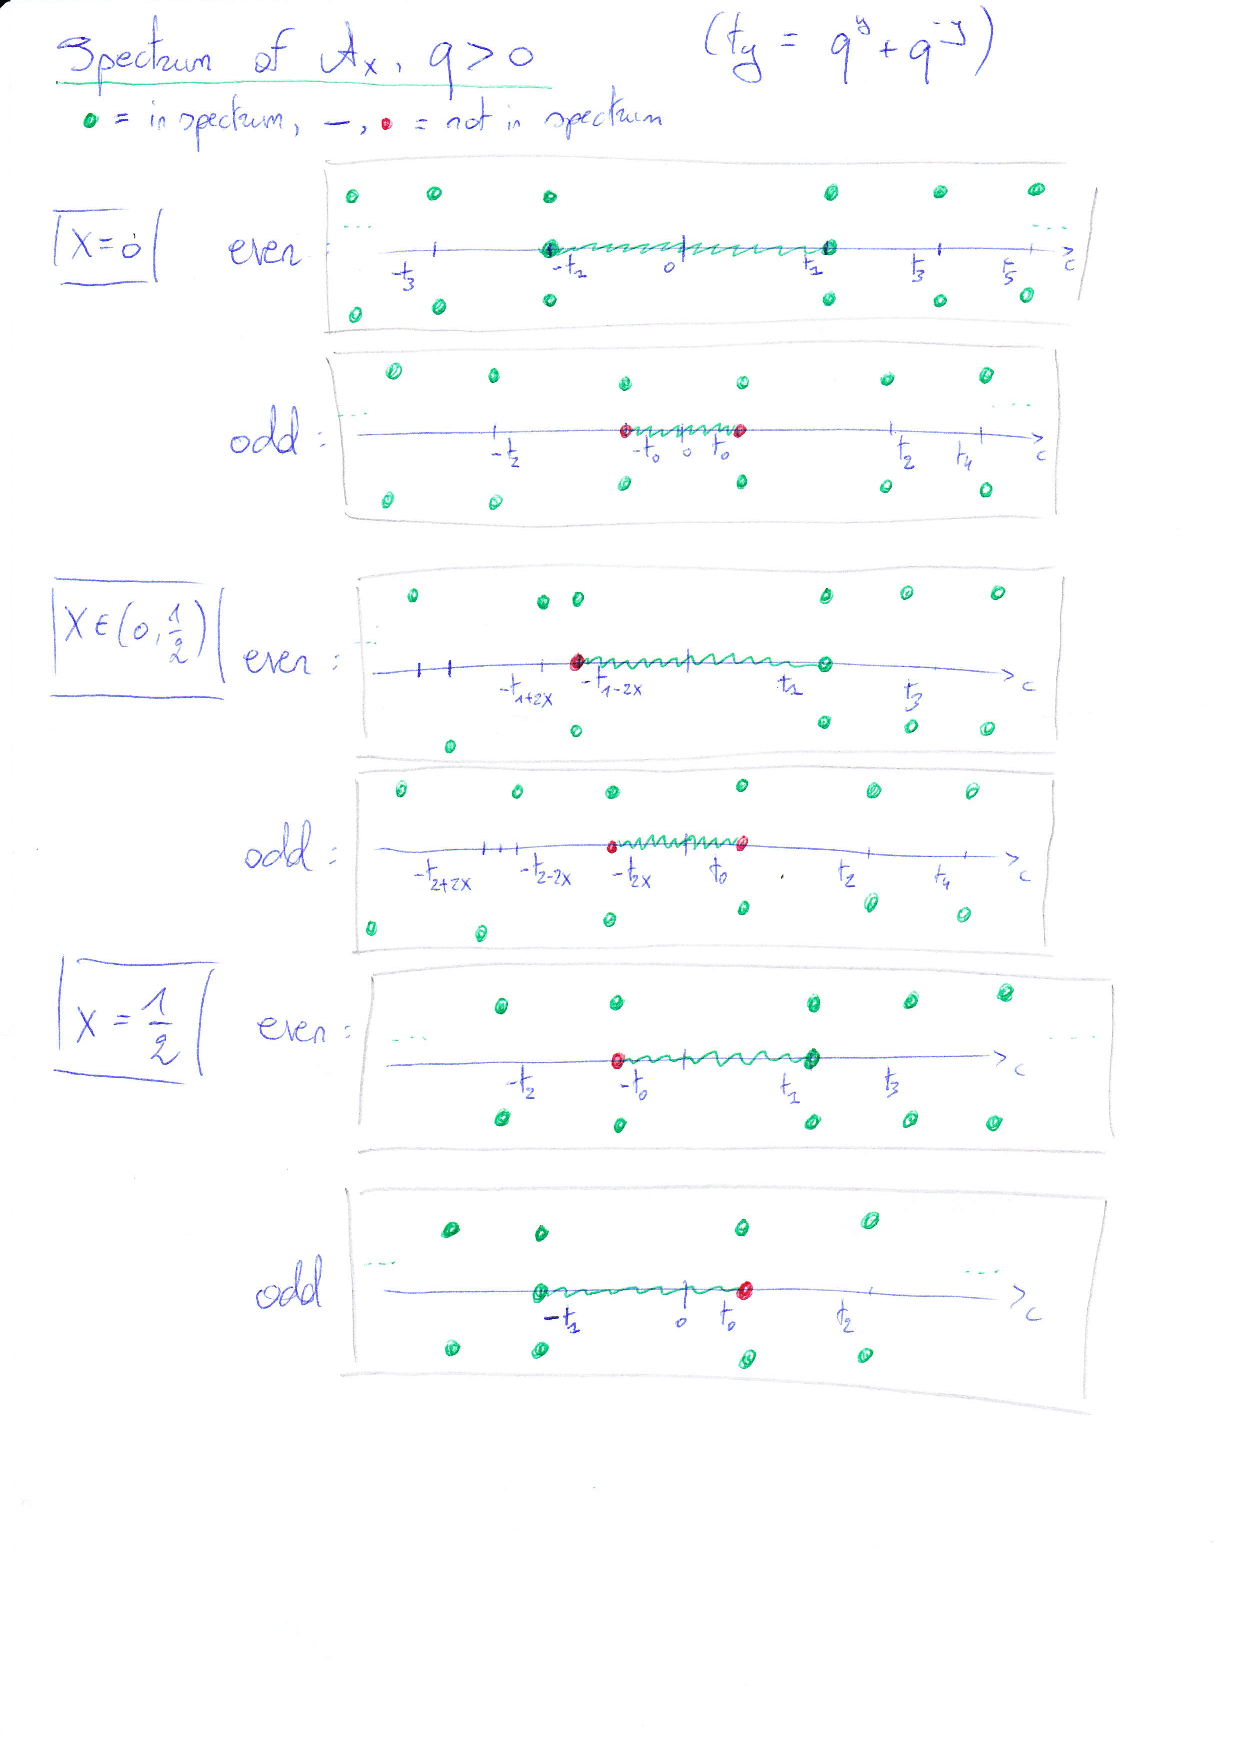
\includepdf[pages={1}]{ScanSpec.pdf}


% Make remark on regular representation cf. Koelink-Rosengren

% Include a concrete descripition of the universal envelope of $A_x$ from this?


%More generally, 

%As a concrete instance of the example of monoidal equivalence, let $\tilde{A}$ be the generalized compact Hopf face algebra obtained from the set $\tilde{I} =I_1\sqcup I_2$ with $I_1= \Z$ and $I_2= \{\bullet\}$ with the $B_{kl} =\emptyset$ and $E(k,l)$ for $k,l\neq \bullet$ as in section ..., with $B_{k,\bullet} = B_{\bullet,k}= \emptyset$, and $B_{\bullet,\bullet} = \{\pm\}$ with $E_{\bullet,\bullet} = \begin{pmatrix} 0 & |q|^{1/2} \\ -\sgn(q)|q|^{-1/2}&0\end{pmatrix}$ (with the basis ordered as $-,+$). Then this will be obtained from the direct sum of the functor from ... and the ordinary forgetful functor from $\Rep(SU_q(2))$ into $\Hilb$. It follows that the components $\tilde{A}(ij)$ can be described by the generators and relations as in ..., but with $F(\lambda)$ and $F(\rho)$ set equal to 1 whenever the corresponding index is $\bullet$.




% Study spectrum fundamental character
% Study dual quantum groupoid
% Make connection with dynamical cocycle
% In case of qgroupoid constructed from identity functor for Rep(SU_q(2)): rep theory of associated Galois object should just be: a single representation (Galois object is type I factor, cutdown of $B(\mathscr{L}^2(SU_q(2)))$). Yes: in general, Galois object is Morita equivalent with algebra of original ergodic action, should also be stressed for Podles spheres

\subsection{The reduced C$^*$-algebra of the dynamical quantum $SU(2)$ group}



% Notation $\weps$ should be recalled?
In \cite{KoR1}, the corepresentation theory of the dynamical quantum $SU(2)$ group is investigated. Transporting their definition to our setting, an $n$-dimensional corepresentation consists of $n^2$ elements $t_{kl} \in M(A_x)$, together with an assigment $k \mapsto q_k \in q^{\Z}$ such that \begin{align*} \Delta(t_{km}) = \Delta(1)\left(\sum_{l=1}^n t_{kl}\otimes t_{lm}\right)&& \weps(t_{kl})\delta_y = \delta_{kl} \delta_{q_ky},&& f(\lambda,\rho)t_{kl} = t_{kl}f(q_k\lambda,q_l\rho).\end{align*} Moreover, the corepresentation is called \emph{unitary} if $S(t_{ij})^* =t_{ji}$. To relate this to the theory of corepresentations defined in \cite{DCT1}, put \[\left(\Gr{t}{y}{z}{v}{w}\right)_{kl} = \delta_{y}(\lambda)\delta_v(\rho) t_{kl} \delta_{z}(\lambda)\delta_{w}(\rho).\] Then this defines a unitary corepresentation in the sense of $\cite{DCT1}$ on the collection of vector spaces $V_{y,z}$ where $V_{y,z}=\{0\}$ except when there exists $k$ with $y = q_kz$,  in which case $V_{y,z} = \mathbb{C}^n$ (and with the matrix coefficients with respect to the canonical basis). 

According to \cite{KoR1}, there is a unitary $2N+1$-dimensional corepresentation $t^N$ for each half-integer $N$ (dropping the tilde appearing in \cite{KoR1}), and moreover the fusion rules of the $t^N$ are as for $SU(2)$. As the tensor products of corepresentations in the sense of \cite{KoR1} and \cite{DCT1} are compatible, we deduce from the abstract theory of \cite{DCT1} that the $t^N$ also form a maximal family of non-equivalent irreducible unitary corepresentations in the sense of \cite{DCT1}. %Moreover, we can label the bases of our vector spaces by integers or halfintegers in such a way that $f(\lambda,\rho)t_{kl}^N = t_{kl}^Nf(q^{-k}\lambda,q^{-l}\rho)$. 
As a concrete example, we have that the generating matrix $(u_{\epsilon,\nu})$ is a unitary corepresentation.

%From the general theory of \cite{DCT1}, we infer that the $\delta_y(\lambda)\delta_z(\rho)t_{kl}^N$ form an orthogonal (but not necessarily orthonormal) basis of $L^2(SU_q(2)_{\dyn})$. 

It then follows straightforwardly from \cite[Section 7]{KoR1} that, with $\varphi_{y,z}$ denoting the Haar functional on $\Gr{A}{y}{y}{z}{z}$, \[\varphi_{y,z}(p(\Omega)) = \int_{\R} p(x)\rd m_{y,z},\] where $m_{y,z}$ is the normalized orthogonality measure for the (rescaled) Askey-Wilson polynomials \[p_k(x) = p_k(2x;qz/y,qy/z,-qyz,-q/yz;q^2).\]  From \cite[Theorem 2.1 and Theorem 2.5]{AsW1}%see also Koelink-Verding
, it follows that $m_{y,z}$ has support on the union of the interval $\lbrack -2,2\rbrack$ with the set \[D_{y,z} = \{\tau(eq^k)\mid e\in \{qz/y,qy/z,-qyz,-q/yz\}, k\geq 0, |eq^k|>1\}.\]

In particular, we deduce the following corollary.

\begin{Cor} The spectrum of $\Omega \,\eta\, \CrG$ equals $\lbrack -2,2\rbrack \cup q^{\Z} \cup (-x^2q^{\Z})\cup (-x^{-2}q^{\Z})$.
\end{Cor} 

In particular, as this spectrum is strictly smaller than the spectrum of $\Omega$ in $\CuG$, we obtain the following theorem.

\begin{Theorem} The partial compact quantum group $SU_q(2)_{\dyn,x}$ is not coamenable.
\end{Theorem} 




%%% Local Variables: 
%%% mode: latex
%%% TeX-master: "dynamical-SUq-file"
%%% End: 
